\documentclass[a4paper,12pt]{article}

\usepackage{natbib,setspace,amsmath,graphicx,float}

\onehalfspacing

\newcommand{\bs}[1]{\boldsymbol{#1}}


\begin{document}


\begin{titlepage}

\noindent
\includegraphics[width=5cm]{uzh_logo_e_pos.pdf}

\noindent{\bf Department of Economics}

\noindent\rule{\textwidth}{0.4pt}

\vspace{1cm}

  \begin{center}
    {\LARGE The Bullionist Controversy}

{\Large Quantitative Economic History - Applications\\Spring Term 2018}

  \end{center}

\vfill

{\flushleft
Name \\
Field of Study\\
Semester\\
Address\\
Phone\\
Email\\
Matriculation Number}  

\end{titlepage}



\pagebreak

\pagebreak
\section{Introduction}

some text: The data can be found in Section \ref{sec:data}

\section{Method}

We estimate a vector autoregressive (VAR) model
\begin{equation}\label{eq:eq1}
    {\bf y}_t={\bf c}+\sum_{j=1}^p{\bf A}_j{\bf y}_{t-j}+{\bf u}_t; \ t=1,2,\ldots,T,
  \end{equation}
where ${\bf y}_t$ is a 2$\times$1 vector containing output growth and inflation.\footnote{See e.g. \citet[Chapter 6]{favero2001}.} To identify supply and demand shocks, we use the implications of a simple AS-AD model and apply the Blanchard-Quah decomposition \citep{blanchardquah89}. Solving the identification problem requires to find the impact matrix ${\bf S}$, which links the structural shocks in $\bs{\epsilon}_t$ to the reduced form residuals in ${\bf u}_t$:
\begin{equation}
  \label{eq:eq2}
  {\bf u}_t={\bf S}\bs{\epsilon}_t.
\end{equation}
The moving-average representation of the reduced-form VAR in equation (\ref{eq:eq1}) is
\begin{equation}
  \label{eq:eq3}
  {\bf y}_t={\bf B}(L){\bf u}_t,
\end{equation}
and for the structural model, we have
\begin{equation}
  \label{eq:eq4}
  {\bf y}_t={\bf C}(L)\bs{\epsilon}_t.
\end{equation}
Because of equation (\ref{eq:eq2}), 
\begin{equation}
  \label{eq:eq5}
  \begin{split}
    {\bf B}(L){\bf u}_t=&{\bf C}(L)\bs{\epsilon}_t;\\
{\bf B}(L){\bf S}\bs{\epsilon}_t=&{\bf C}(L)\bs{\epsilon}_t;\\
{\bf B}(L){\bf S}=&{\bf C}(L).
  \end{split}
\end{equation}
The relationship between the long-run multipliers is
\begin{equation}
  \label{eq:eq6}
  {\bf B}(1){\bf S}={\bf C}(1).
\end{equation}
Therefore, to find ${\bf S}={\bf B}(1)^{-1}{\bf C}(1)$, we need ${\bf C}(1)$.

Pre- and postmultiplying the variance-covariance matrix $\bs{\Sigma}$ of the reduced form residuals ${\bf u}_t$ with ${\bf B}(1)$ and its transpose gives
\begin{equation}
  \label{eq:eq7}
  \begin{split}
  {\bf B}(1)\bs{\Sigma}{\bf B}(1)^{\prime}=&{\bf C}(1){\bf S}^{-1}\bs{\Sigma}({\bf S}^{\prime})^{-1}{\bf C}(1)^{\prime}=\\=&{\bf C}(1){\bf S}^{-1}{\bf S}{\bf S}^{\prime}({\bf S}^{\prime})^{-1}{\bf C}(1)^{\prime}=\\=&{\bf C}(1){\bf C}(1)^{\prime}.
      \end{split}
\end{equation}
If we assume a lower-triangular structure for ${\bf C}(1)$,\footnote{Output is only affected by supply shocks, while the price level reacts to both demand and supply shocks.} we can use the Cholesky decomposition of ${\bf B}(1)\bs{\Sigma}{\bf B}(1)^{\prime}$ to recover ${\bf C}(1)$.

\section{The Data\label{sec:data}}

\begin{itemize}
\item Price index:
\begin{itemize}
\item 1700-1823: \citet{schumpeter38}, in \citet[p. 468-469]{mitchelldeane71}
\item 1823-1913: \citet[p. 863-864]{mitchelle2003}
\end{itemize}

\item Industrial production: \citet[p. 725-727]{craftsharley92}

\end{itemize}

\section{Results}

\begin{figure}[H]
    \centering
\caption{Impulse Responses}
    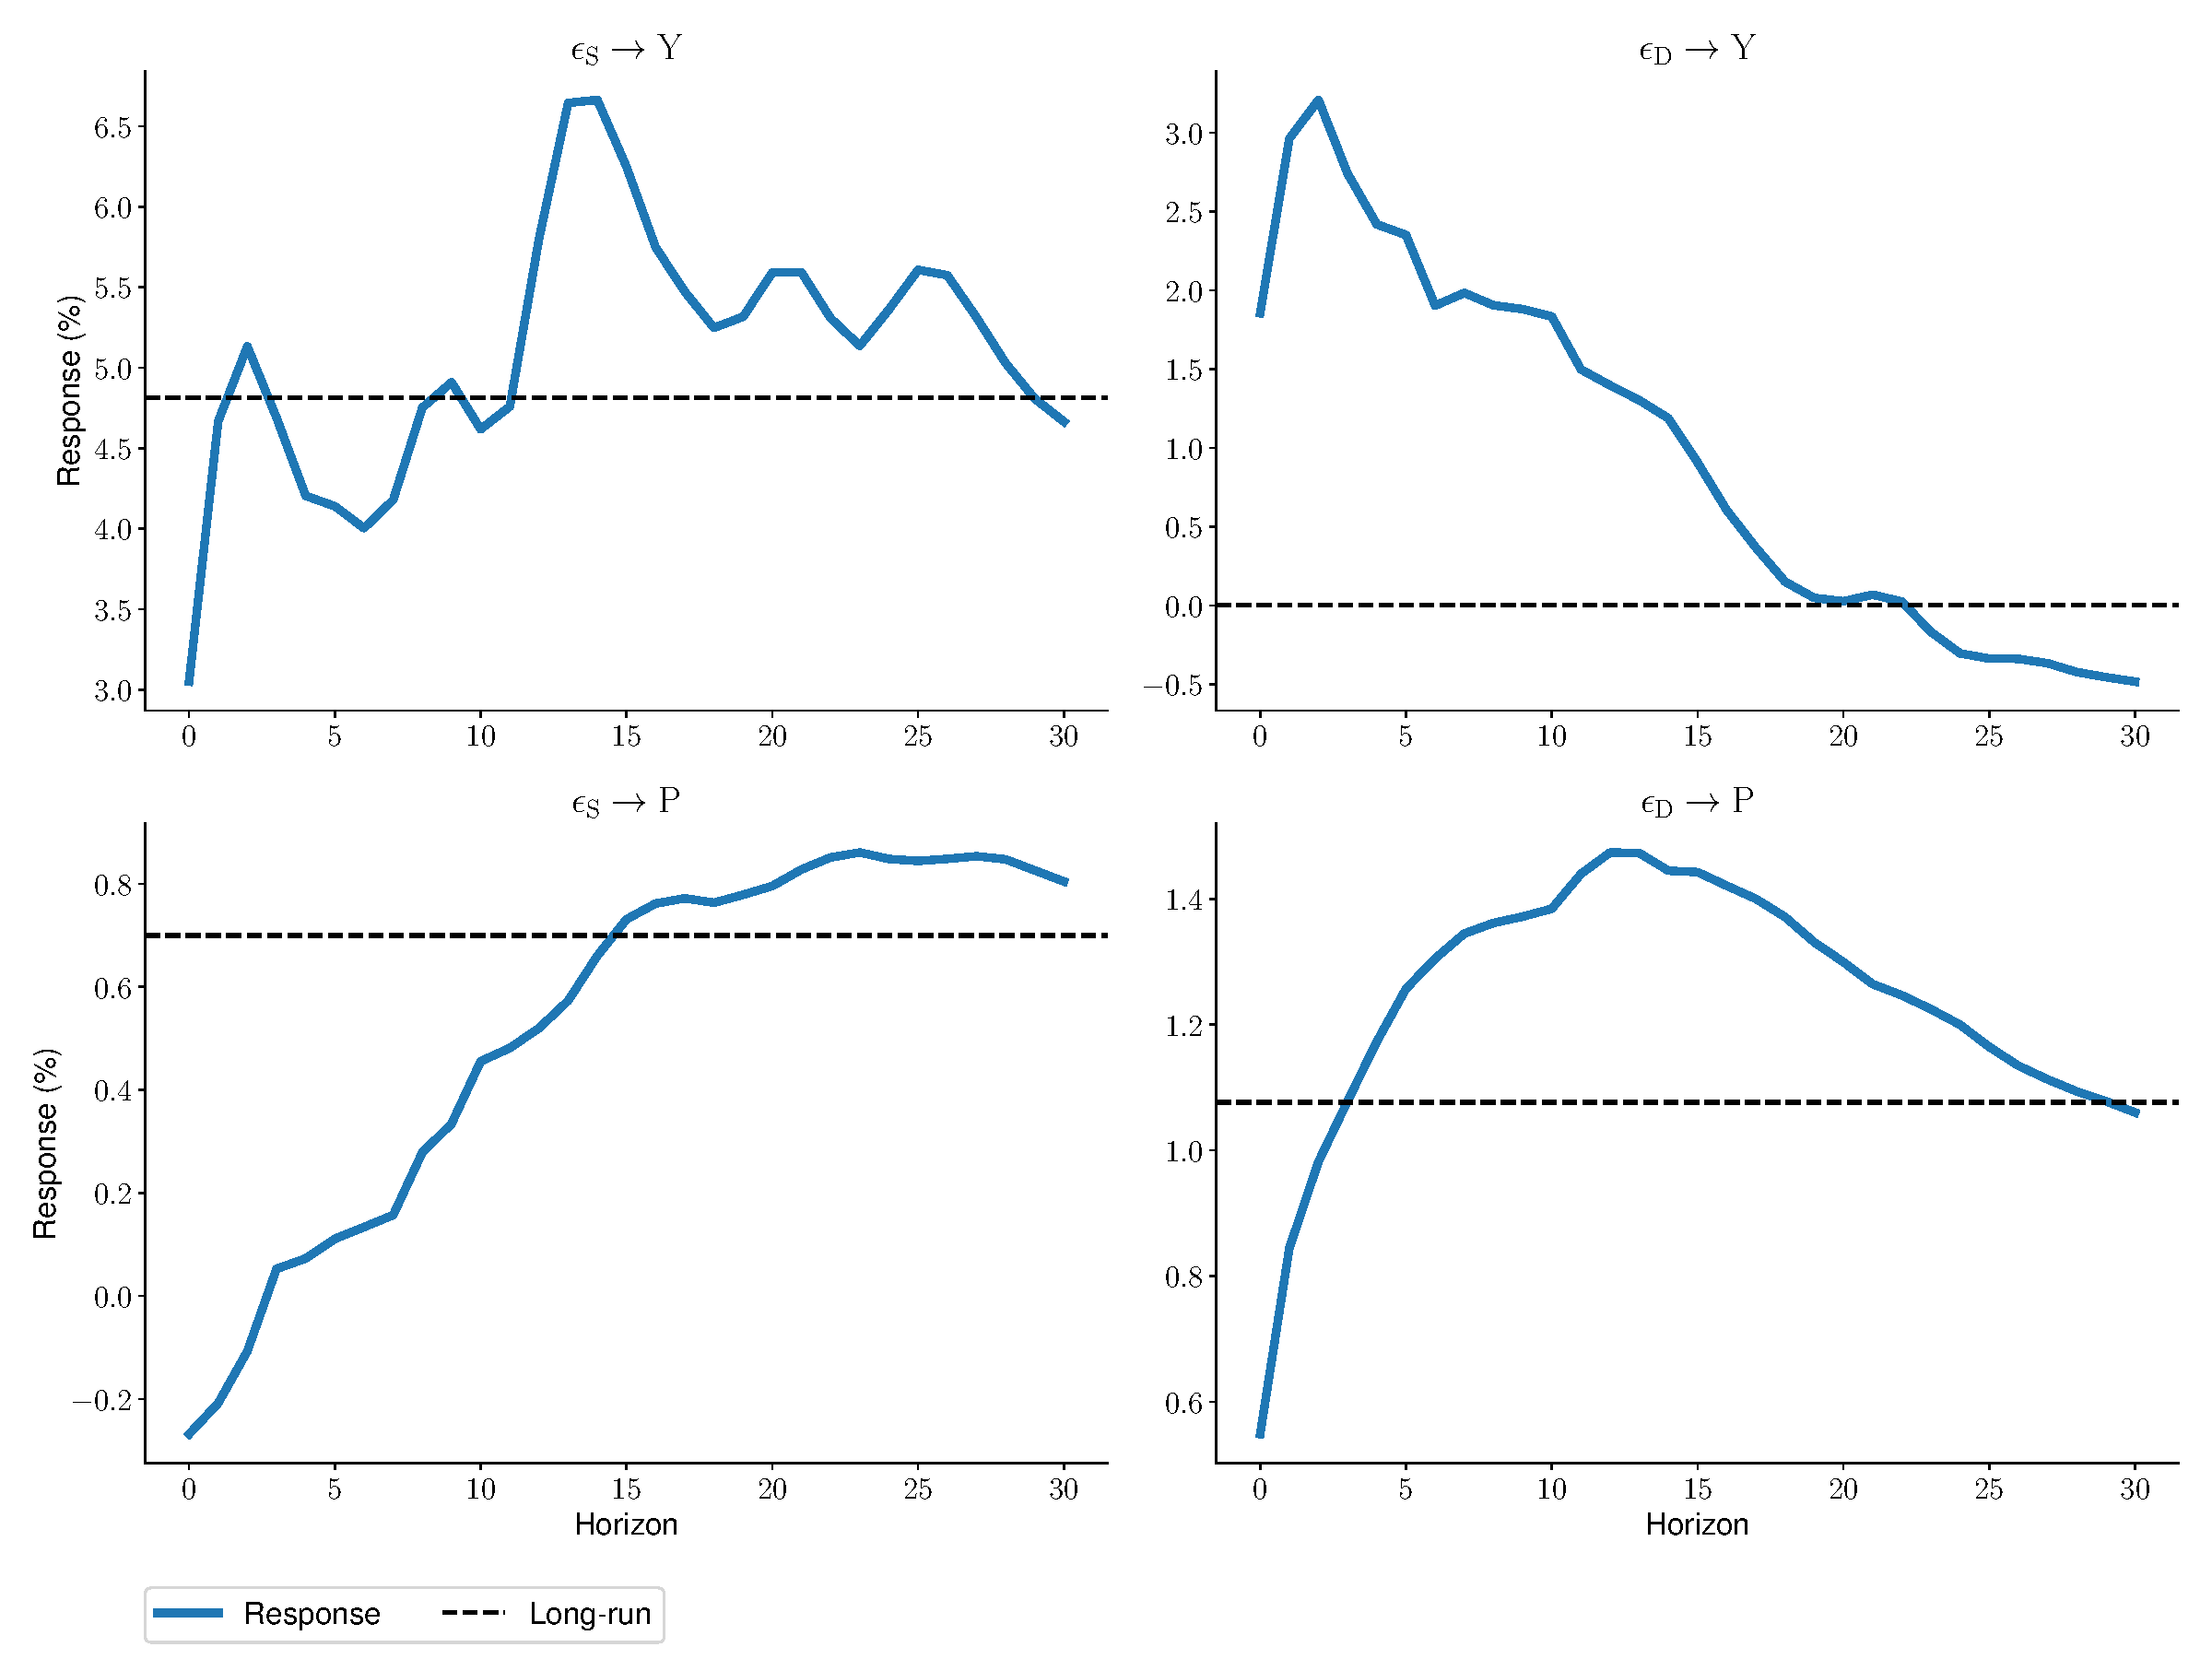
\includegraphics[width=\textwidth]{../output/figures/IR.pdf} 
\end{figure}

To be discussed.

\pagebreak

\bibliography{sqwg}
\bibliographystyle{eeh}

\end{document}
